
%\documentclass[twocolumn,letterpaper]{article}
\documentclass[10pt]{csce}

\usepackage[hmargin=.75in,vmargin=1in]{geometry}
\usepackage[american]{babel}
\usepackage[T1]{fontenc}
\usepackage{times}
\usepackage{caption}
\usepackage{flushend}

\usepackage{gensymb,hyperref,graphicx,paralist,amsmath,multirow}
\usepackage[table]{xcolor}
\pagenumbering{gobble}

\title{\bf A Model-Based Scheduling Framework for Enhancing Robustness}

%%%% Make sure the author names are boldface.
\author{
{\bfseries Nicolas Grounds and John K. Antonio}\\
School of Computer Science, University of Oklahoma, Norman, Oklahoma, United States of America\\
}

\begin{document}

\maketitle                        %%%% To set Title and Author names.

\begin{abstract}
In previous work the performance of scheduling algorithms for dynamic
scheduling of tasks in a distributed system were evaluated for their
robustness to error in the model of tasks' information.  There it was
found that incorporating task completion timings from the actual distributed
system into the algorithms' model of the system was crucial for achieving
robustness.  In this paper, various degrees of feedback, rather than simply
all-or-none, are evaluated using the same simulated studies as in previous
work and a proposed strategy for biasing model tasks' information is proposed
in order to counteract the most egregious effects of model error on
performance.
\end{abstract}


\vspace{1em}
\noindent\textbf{Keywords:}
 {\small distributed system, scheduling, performance, robustness, biasing}


\section{Introduction and Background}
\label{sec:Intro}

Scheduling computational tasks to machines so as to improve specified metrics
of performance has been the topic of a plethora of good work produced over the
past several decades \cite{taxonomy}. The underlying assumptions and objectives
of this body of work varies along several dimensions. First, some work assumes
all tasks are independent whereas other work, as in this paper, allows for
tasks to have dependency or precedence relationships with other tasks (for
which interrelated tasks are typically represented in a directed acyclic graph,
or DAG). Additionally, there are static formulations to scheduling in which a
desired schedule is detemined offline based on assumed knowledge related to the
machines' available resources and, correspondingly, the resource requirements
of the computational tasks.

Conversely, this paper addresses dynamic scheduling in which the schedule for
tasks is determined online in real-time with the execution of those tasks on a
distributed system. Unlike the static scheduling problem, dynamic scheduling
does not require upfront knowledge of the arrival of future tasks into the
system for scheduling. Algorithms for dynamic scheduling make use of knowledge
about the tasks which are ready for scheduling and their resource requirements
such as CPU and memory load as well as the resource capacities of the machines
in the distributed system.

Such algorithms for dynamic scheduling may be based on heuristics for selecting
which tasks to prioritize execution of and determining when to begin their
execution and on which machine. Other algorithms may actively attempt to
optimize scheduling decisions with respect to a desired outcome based on a
user-defined objective.  Both types of algorithms are generally measured
and compared to one another against such objectives such as minimizing makespan
(time required for completed execution of all tasks) \cite{stochastic}, or, as
in this paper, the degree to which all tasks of a DAG are completed by a
DAG-associated deadline.

Scheduling algorithms may orthogonally be evaluated based on their robustness,
for example, how well the same objective is achieved when information provided
to the scheduling algorithm contains errors such as inaccuracies in the
amount of resource requirements of the tasks.  In previous work \cite{pdpta18}
four dynamic scheduling algorithms' robustness to error with respect to
performance against an objective of completing DAGs before their deadline was
presented, showing how some algorithms were not robust to even the smallest
amount of simulated error.  Additionally, the use of task completion time
feedback from the actual distributed system back into the modeled system used
by the scheduling algorithms was found to substantially improve robustness of
all four scheduling algorithms to even large amounts of simulated error.

The remainder of the paper is organized in the following manner.  Section
\ref{sec:Framework} describes the problem domain and the simulation software's
use of modeling the distributed system where errors in task requirements may
be inherent.  Section \ref{sec:Biasing} presents an approach to counteracting
model error to prevent scheduling algorithms from over-committing system
resources to executing too many tasks concurrently. Section \ref{sec:Results}
presents results of simulated case studies within that software simulator.
Finally, Section \ref{sec:Summary} summarizes the findings from these
simulations and presents the conclusions of our work.


\section{Problem Domain and Simulation Environment}
\label{sec:Framework}

The present work is a meta-approach that is motivated by the desire to apply
existing scheduling approaches within a framework that is realistic and
operationally practical.  In terms of scheduling taxonomy, we assume a dynamic
scheduling formulation in which the computational jobs (we call them workflows)
are modeled as directed acyclic graphs, i.e., the tasks of a workflow have
precedence constraints.  Furthermore, each workflow (not individual tasks) is
endowed with a deadline. 

Our framework, illustrated in Figure \ref{fig:platform}, consists of one
centralized scheduler and two instances of the computational platform.  The
first instance, denoted as the actual platform, represents the actual machines
(virtual or physical) upon which the actual workflows' tasks are to be executed.
The second instance of the platform, denoted as the model platform, is a
mathematical and/or simulated model representation of the actual platform.  The
scheduler component makes decisions about what machine each task is to be
executed on and when (at or after all the tasks precedence constraints are
satisfied) that execution should begin.  The scheduler makes use of a scheduling
algorithm, which requires some model of the workflows' tasks' requirements.
Scheduling decisions are implemented by a task assigner particular to the
platform, model or actual.

\begin{figure}
	\begin{center}
		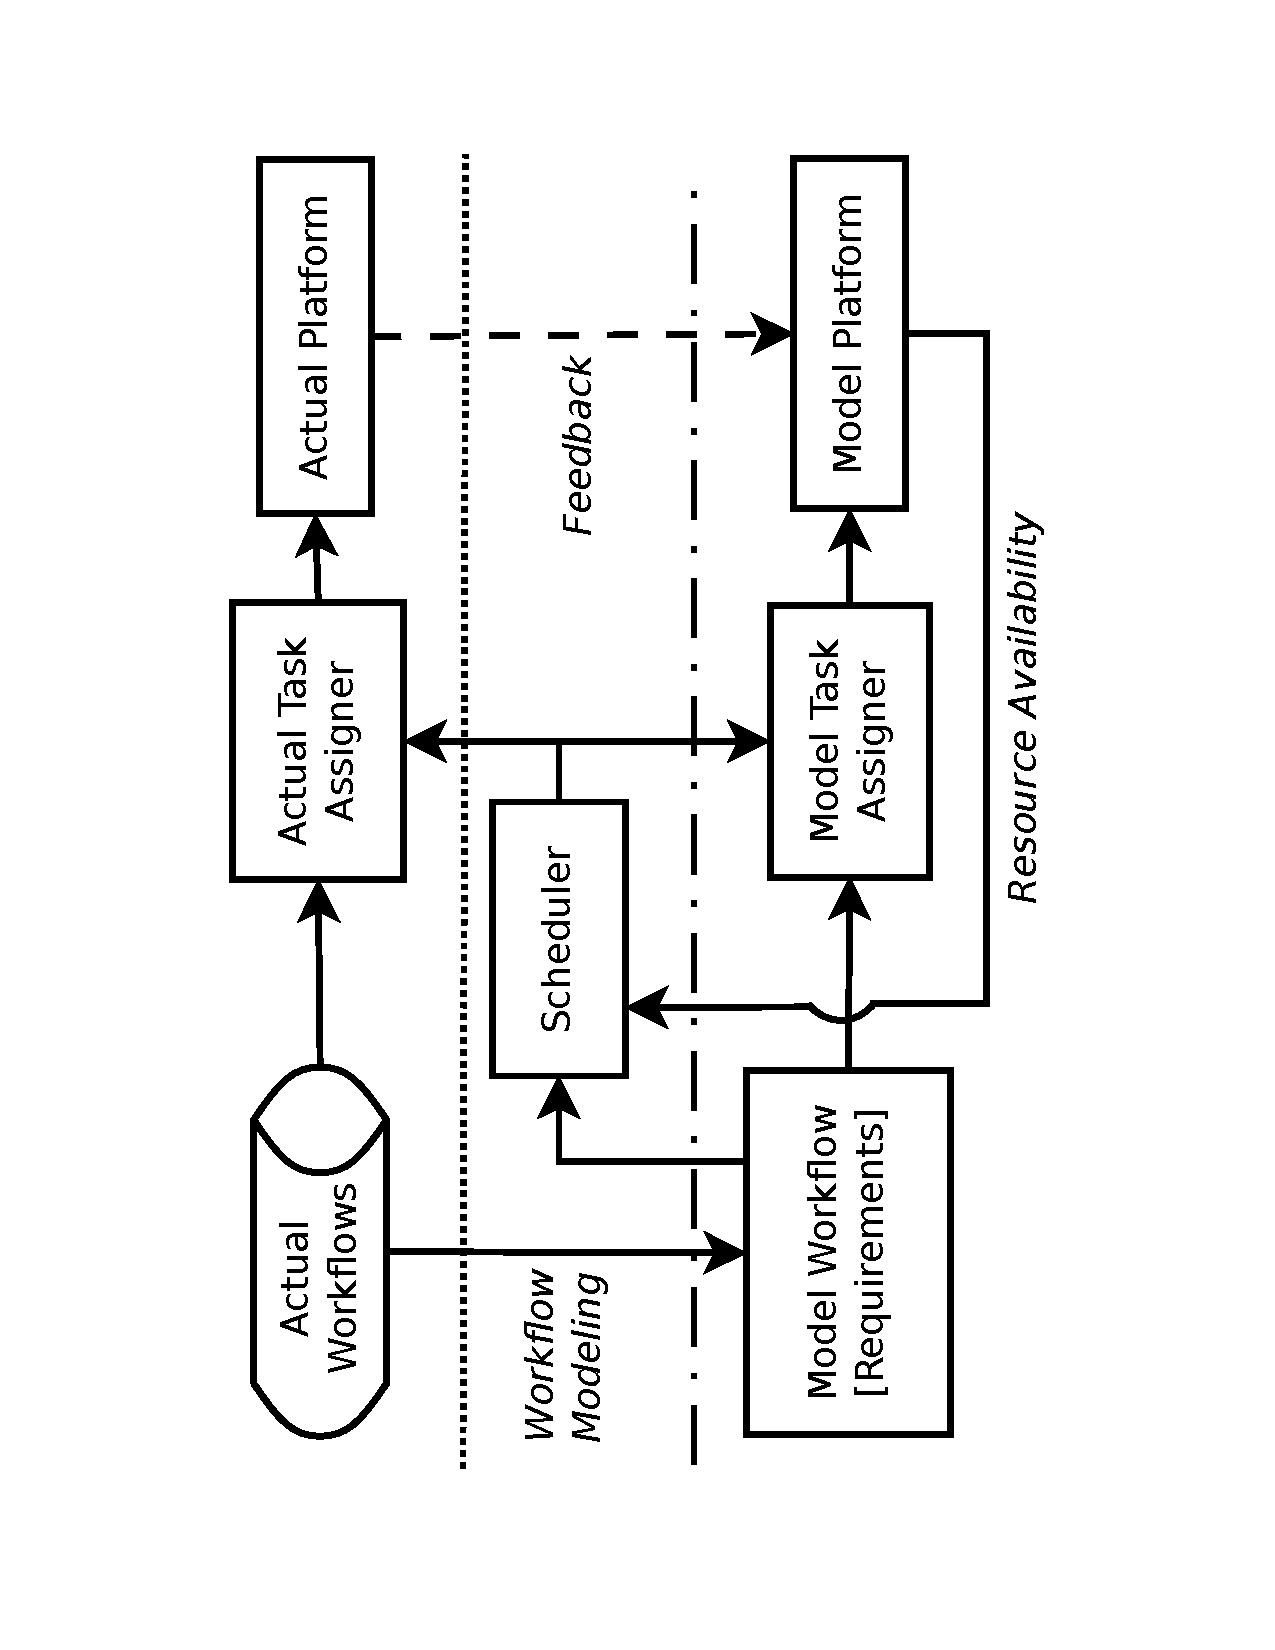
\includegraphics[angle=-90,width=0.5\textwidth]{figures/PlatformDiagram.pdf}
	\end{center}
	\caption{Block diagram illustrating proposed framework.}
	\label{fig:platform}
\end{figure}

Much past research has focused on the scheduler component of Figure
\ref{fig:platform}; building schedulers to achieve enhanced performance and/or
robustness.  This is often achieved by focusing on the modeled workflow's
rquirements information provided to the scheduler.  In addition to modeling
requirements, our framework also emphasizes modeling of the platform resources
through the model platform component, providing additional opportunities for
research and improvement.  Such improvements can be realized by building more
accurate models or by making use of feedback from the actual platform to correct
the model platform, indicated by the dashed line of Figure \ref{fig:platform}.

Development and evaluation of static schedules, and schedulers, make use of the
components below the dotted line to build a schedule (set of scheduling
decisions for where and when each task should be executed).  That static
schedule is then used by the actual task assigner component, e.g., via a lookup
table, in a running system like that represented above the dotted line.  Also,
for scheduling algorithms that require training, or offline optimization of
parameters, the same components below the dotted line would be used prior to
deployment of the algorithm in the scheduler of a live system, represented
by the components above the dashed-dotted line.

In the ideal case that the model components match the behavior of the
corresponding actual components, feedback from the actual platform is
unnecessary. Realistically, however, the model components will have deviations
(or errors) in comparison to the actual components with how they
model the tasks' requirements and the availability of platform resources.  This
leads to erroneous information being presented to the scheduler that can be
summarized as two interrelated types.  First, task requirement error results in
inaccurate information about resource load in the model platform, which is
utilized by the scheduler.  Because all scheduling algorithms must fundamentally
determine when to schedule additional tasks on already-loaded resources versus
when to delay starting new tasks until some already-running tasks complete and
the load of the resources lightens (increasing its efficiency), an algorithm
given wrong information about resource load will generally make poor
decisions.

The second type of error the model may exhibit is in the representation of
how much work a task requires to be completed before the task is considered
finished.  When a model's error causes a task's work requirement to be
underestimated, it can lead the scheduling algorithm to assign additional
work to the resource modeled as now having a lightened load.  In this scenario
the error compounds if the algorithm assigns new tasks to the resource because
the additional load causes the atual system's resource to become even less
efficient, further diverging the model from the actual system and causing the
task erroneously modeled as finished to take even longer to finish in the
actual system.  It is also possible that the model for a task overestimates
the task's work requirement in which case the model of the resource remains
loaded while the actual system's resource may be idle.

To counteract the effect of the model diverging from the actual system in
terms of knowledge of which tasks are running, the model may be improved
using feedback from the actual system regarding task completion.  A simple
implementation of this feedback in practice is to instrument the actual system
to provide periodic information about the running tasks on each system
resource.  However, this can cause the model to `lag' behind the actual system
if modeled tasks are not considered completed until a periodic check reveals
its actual system counterpart is no longer executing.  Because scheduling
algorithms make decisions once the state of the system changes in response to
tasks finishing, the aforementioned `lag' may be avoided by having the actual
system provide event-based feedback upon completion of each task.  This latter
`event-driven' approach is adopted in our framework.


\section{Use of Biasing}
\label{sec:Biasing}

This section presents simulated results of the outcomes of scheduling algorithms
whose decisions are made based on a model platform of the (simulated) actual
system in which error is introduced in one aspect of the workflows' tasks'
requirements.  It is shown that by using actual task completion events (fed back
from the actual platform) to correct inaccuracies present in the model
platform, all scheduling algorithms analyzed become very robust to errors in the
tasks' requirements considered.

All simulations were performed using simulator software developed for
previous research \cite{costmin} and made publically available as open source
\cite{soasim}.  As in \cite{costmin} workflows are defined as a directed
acyclic graph where graph nodes represent the computational tasks which are
individually schedulable to execute on one of the platform's available machines.
Graph edges represent precedence constraint where one task must complete
execution before the connected task is able to be scheduled and begin
execution.  In every simulation a scheduling algorithm
is used to schedule tasks from arriving workflows of one of three types, as
also defined in \cite{costmin}: small workflows representative of simple
interactive application jobs, medium workflows representative of web services
jobs, and large workflows representative of large-scale batch-oriented jobs.
Various workflow and task characteristics are summarized in Table
\ref{tab:params}.

\begin{table}
	\begin{tabular}{|l|c|c|c|}
		\hline
		\textbf{Parameter}	& \textbf{Small}	& \textbf{Medium}	& \textbf{Large} \\
		\hline
		Total tasks				& [5,16]	& [10,72]	& [45,800] \\
		Potential Task Parallelism	& [1,2]	& [2,3]		& [5,20] \\
		Task CPU cycles (work)	& [1,2.5]	& [10,50]	& [50,175] \\
		Task CPU utilization	& [0.5,1]	& [0.5,1]	& [0.5,1] \\
		Task memory footprint	& [0.05,0.15] & [0.05,0.1] & [0.05,0.1] \\
		\hline
	\end{tabular}
	\caption{Table of basic workflow (DAG) sizes and tasks' requirements by
		workflow type.}
	\label{tab:params}
\end{table}

As part of the simulation studies the model workflows are given task
requirements where the tasks' amount of CPU cycles ($C_M$) to be completed has
an error term applied to it with respect to the actual value ($C_A$).
This error term parameter $X$ is varied between experiments from 0.001 to 0.9.

\begin{equation}
\begin{split}
C_M & \leftarrow (1+x)C_A \\
x & \in [-X,X]
\end{split}
\end{equation}

\noindent The values for $x$ drawn from $[-X,X]$ assume a uniform distribution.

As with \cite{costmin} all simulations used a simulated platform of 16 machines
with the same resource capacities: $4$ CPUs and a normalized memory capacity of
$1.0$.  From Table \ref{tab:params}, then, each task would consume between half
and all of a single CPU and between $5\%$ and $15\%$ (for small workflows, or
$10\%$ for medium and large) of total memory.  For all numeric results for
$10\%$ for medium and large) of total memory.  Platform machine efficiency was
simulated the same as in \cite{costmin} where cumulative CPU load of all
executing tasks on a machine, $\ell_c$, resulted in an effiency, $e_c$ given in
Eq. \ref{eq:cpueff}.  Memory effiency, $e_m$, based on cumulative memory
load of all executing tasks, $\ell_m$, is given in Eq. \ref{eq:memeff}.
The combined efficiency, $e = e_c e_m$, represents the amount of work
accomplished on each executing task per unit of time.


\begin{equation}
\label{eq:cpueff}
e_c = \begin{cases}
	1, ~~~~~~~~\ell_c < 4 \\
	(4/\ell_c), ~~\ell_c \ge 4
\end{cases}
\end{equation}

\begin{equation}
\label{eq:memeff}
e_m = \frac{10}{10 + \frac{1}{(1/\ell_m) - 1}}
\end{equation}

For all numeric results for
performance the value presented is an averaged value across ten simulations
where the workflows and tasks were the same but a unique random error term,
$x$, was used for each model task's required CPU cycles.

\begin{figure*}
	\begin{center}
		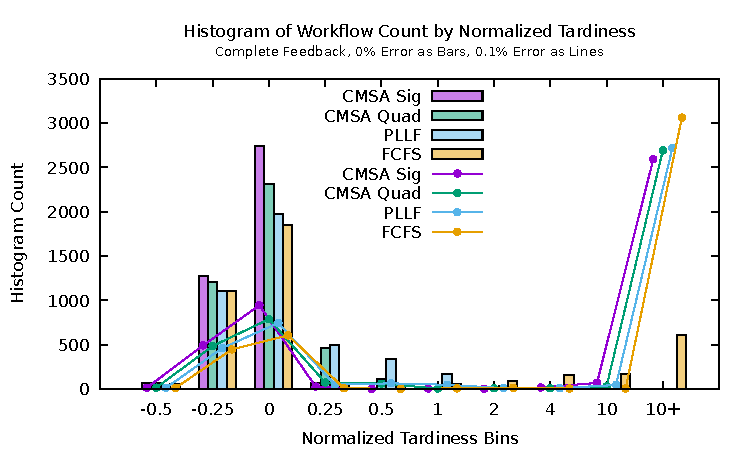
\includegraphics[width=0.9\textwidth,height=3in]{figures/Histogram_All_NoLoss_NoBias_LowError.pdf}
	\end{center}
	\caption{Histogram of workflows by normalized tardiness comparing
		relative performance of scheduling algorithms with no error (vertical
		bars) and with 0.1\% error applied to the model of the workflow
		requirements (line graphs).  In this scenario, task completion event
		feedback was \textbf{not} employed to correct the model platform.}
	\label{fig:noloss-lowerror-nofeedback}
\end{figure*}


\section{Results}
\label{sec:Results}

Figure \ref{fig:noloss-lowerror-nofeedback} shows the performance of scheduling
algorithms and the significant performance impact that even a small amount of
error has.  In this figure as with prior research, performance is depicted
visually as a histogram of the number of workflows completed in intervals based
on their normalized tardiness (the time difference between the completion and
the target deadline normalized by on-time completion time of the workflow).
In this representation a normalized tardiness of 0 represents a workflow that
completed exactly at its deadline, negative values represent workflows completed
before their deadline, and positive values those completed late.

The histogram bars of Figure \ref{fig:noloss-lowerror-nofeedback} represent the
performance of scheduling algorithms under the ideal circumstance of no error
in the model (i.e., the model platform perfectly predicts and represents the
resources required by a task and its execution completion time).  These
histogram bar results demonstrate how CMSA with either of the two
cost functions (Sigmoid or Quadratic) completes the largest majorities of
workflows ahead of their deadline.  The PLLF (proportional least laxity first)
algorithm completes workflows up to 4 times later (as a proportion of the
ideal finish time) than the deadline. The FCFS (first-come, first-serve)
algorithm performs relatively poorly with workflows completing far later than
their deadline because it is oblivious to deadlines and therefore often will
put off scheduling tasks of a recently-arrived workflow with a `tight' deadline
by prioritizing a less-recently arrived workflow despite its deadline being
further into the future and possibly more relaxed.

The lines graphed in Figure \ref{fig:noloss-lowerror-nofeedback} represent the
same algorithms' histogram of workflow completion in the presence of 0.1\% error
in the model platform.  As depicted, one algorithm (CMSA algorithm optimizing
the cost based on a Sigmoid cost function) maintains roughly the same
performance in the presence of this small model error, as without it.  All three
other algorithms exhibit a dramatic loss in performance, i.e., a shift of many
workflows completing ahead of or shortly after their deadline to completing
many times over later than their deadline.  In this scenario, completion events
were \textbf{not} employed to correct the model platform.

\begin{table}
       \begin{center}
       \begin{tabular}{lllll}
\textbf{Error, }$X$ & \textbf{CMSA}	& \textbf{CMSA}				& \textbf{FCFS}				& \textbf{PLLF} \\
		& \textbf{(Quad)}			& \textbf{(Sig)}			&							& \\
0.0		& \cellcolor{red! 6}16.54	& \cellcolor{green!9}1.77	& \cellcolor{red!28}38.49	& \cellcolor{red!28}38.72 \\
0.001	& \cellcolor{red!20}30.52	& \cellcolor{green!9}1.92	& \cellcolor{red!51}61.39	& \cellcolor{red!40}50.96 \\
0.005	& \cellcolor{red!24}34.75	& \cellcolor{green!9}1.84	& \cellcolor{red!49}59.48	& \cellcolor{red!42}52.39 \\
0.01	& \cellcolor{red!20}30.86	& \cellcolor{green!7}2.99	& \cellcolor{red!50}60.35	& \cellcolor{red!39}49.39 \\
0.05	& \cellcolor{red!18}28.87	& \cellcolor{green!1}8.99	& \cellcolor{red!53}63.60	& \cellcolor{red!39}49.54 \\
0.1		& \cellcolor{red!22}32.11	& \cellcolor{red! 5}15.60	& \cellcolor{red!50}60.77	& \cellcolor{red!42}52.65 \\
0.5		& \cellcolor{red!24}34.34	& \cellcolor{red!14}24.96	& \cellcolor{red!42}52.85	& \cellcolor{red!45}55.68 \\
0.9		& \cellcolor{red!22}32.93	& \cellcolor{red!16}26.12	& \cellcolor{red!44}54.36	& \cellcolor{red!48}58.64 \\
       \end{tabular}
       \caption{Percent of workflows late for four scheduling algorithms
			across various amounts of error in the model platform.  Completion
			events were \textbf{not} employed to correct the model platform.}
       \label{tab:perclate}
       \end{center}
\end{table}

Table \ref{tab:perclate} lists the value of percent of all workflows completed
late (after their deadline) as a single performance metric for the scheduling
algorithms across various amounts of the error term, $X$.  This metric (percent
late workflows) is useful in comparing the impact of increasing error on the
performance of each scheduling algorithm.  Like Figure
\ref{fig:noloss-lowerror-nofeedback}, it illustrates how CMSA (with sigmoid cost
function) is robust to small error, whereas the other algorithms are not.  It
also shows that while the performance of CMSA (Sig) degrades as error increases,
the other three algorithms maintain nearly a constant level of even poorer
performance with any amount of error.  These results show how some algorithms
(CMSA with Sigmoid cost function) can be relatively robust (at least with
respect to this performance metric) for small amounts of error but how all
algorithms eventually perform poorly when using a model platform that fails to
reasonably represent the actual system.

The model task requirement with respect to the amount of CPU cycles each task
requires has a compounding effect when the model system declares, erroneously,
that a task has completed (ahead of the actual system) and thus the scheduler
determine to begin execution of an additional task that increases the system
resource load in the actual system and slows the progression toward completion
even further.  Intuitively, this compounding error is most likely the reason
for such a dramatic decrease in overall scheduler performance for the three
affected algorithms of Figure \ref{fig:noloss-lowerror-nofeedback}.

\begin{figure*}
	\begin{center}
		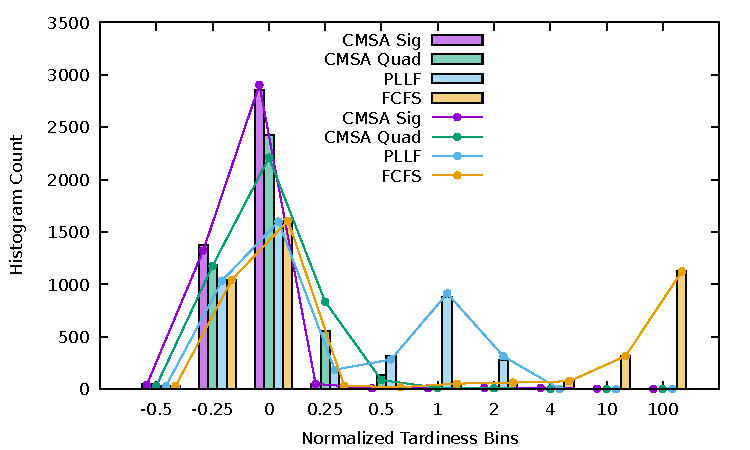
\includegraphics[width=0.9\textwidth,height=3in]{figures/Histogram_All_NoLoss_NoBias_HighErrorWithoutModelFinishEvents.pdf}
	\end{center}
	\caption{Histogram of workflows by normalized tardiness comparing relative
		performance of scheduling algorithms with no error (vertical bars) and
		with 90\% error applied to the model of the workflow requirements
		(line graphs).  In this scenario, task completion event feedback
		\textbf{was} employed to correct the model platform.}
	\label{fig:noloss-higherror-nomodel}
\end{figure*}

The strategy proposed in this paper is to incorporate feedback from the actual
platform for task completions as an event-based trigger for updating the
model platform and allowing the scheduler to schedule new tasks.  Figure
\ref{fig:noloss-higherror-nomodel} depicts results of the performance of
scheduling algorithms comparable with Figure
\ref{fig:noloss-lowerror-nofeedback} except that the error introduced in the
model is much higher (90\%, instead of 0.1\%) and the model platform uses task
completion events from the actual platform (instead of relying on the model
platform estimates of task completions).  Given that the line graphs match
much more closely to the vertical bars than in Figure
\ref{fig:noloss-lowerror-nofeedback}, this illustrates how even for large
model error the incorporation of actual platform task completion feedback
increases the robustness of all four scheduling algorithms.  The CMSA (Sig)
algorithm which was robust for small amounts of error, as well as the other
three algorithms which were not robust even for the smallest amount of error
studied (0.1\%) all achieve nearly the same level of performance (i.e. shape
of histogram) as with having a perfect, no-error model.


\section{Summary and Future Work}
\label{sec:Summary}

In this paper we introduced a framework for understanding and evaluating
scheduling algorthms' performance and robustness with
respect to error in tasks' resource requirements.  This framework
incorporates a model of the actual system in which errors and uncertainties can
be represented.  Through simulation studies we examined the performance of four
scheduling algorithms and the impact of error in the model system upon their
performance.  While the CMSA algorithm (using a sigmoid cost function) had some
degree of robustness, i.e. it was able to achieve similar performance in the
presence of very small error, all algorithms exhibited poor performance with
even moderate amounts of error present in one dimension of the model workflows
requirements (CPU cycles required for the tasks).

We also introduced and simulated the notion of incorporating feedback from
the actual system back into the model system.  Through simulation studies we
showed how all algorithms can benefit from feedback of task completion events
and thus become relatively robust to even substantial error in the model
system.

In the present paper, we assumed that tasks' completion events are detected
and fed back in order to `correct' the model platform.  Under this
assumption, the model completely relies on actual completion events being
fed back.  Future work will consider the possibility in which partial feedback
(of some) completion events are available and fed back to the model.  This
`partial feedback' assumption may be more practical than the complete feedback
used in this paper in situations where there would be significant overhead
instrumenting the actual system so as to feed back each and every completion
event.  In such cases, taking small samplings of completion events from the
actual system would be more practical. Finally, future work will also
investigate the effect of non-uniform error and/or error distributions without
an expected value of $0$.

\bibliography{paper}{}
\bibliographystyle{unsrt}

\end{document}

